\begin{figure*}
\centering
  \centering
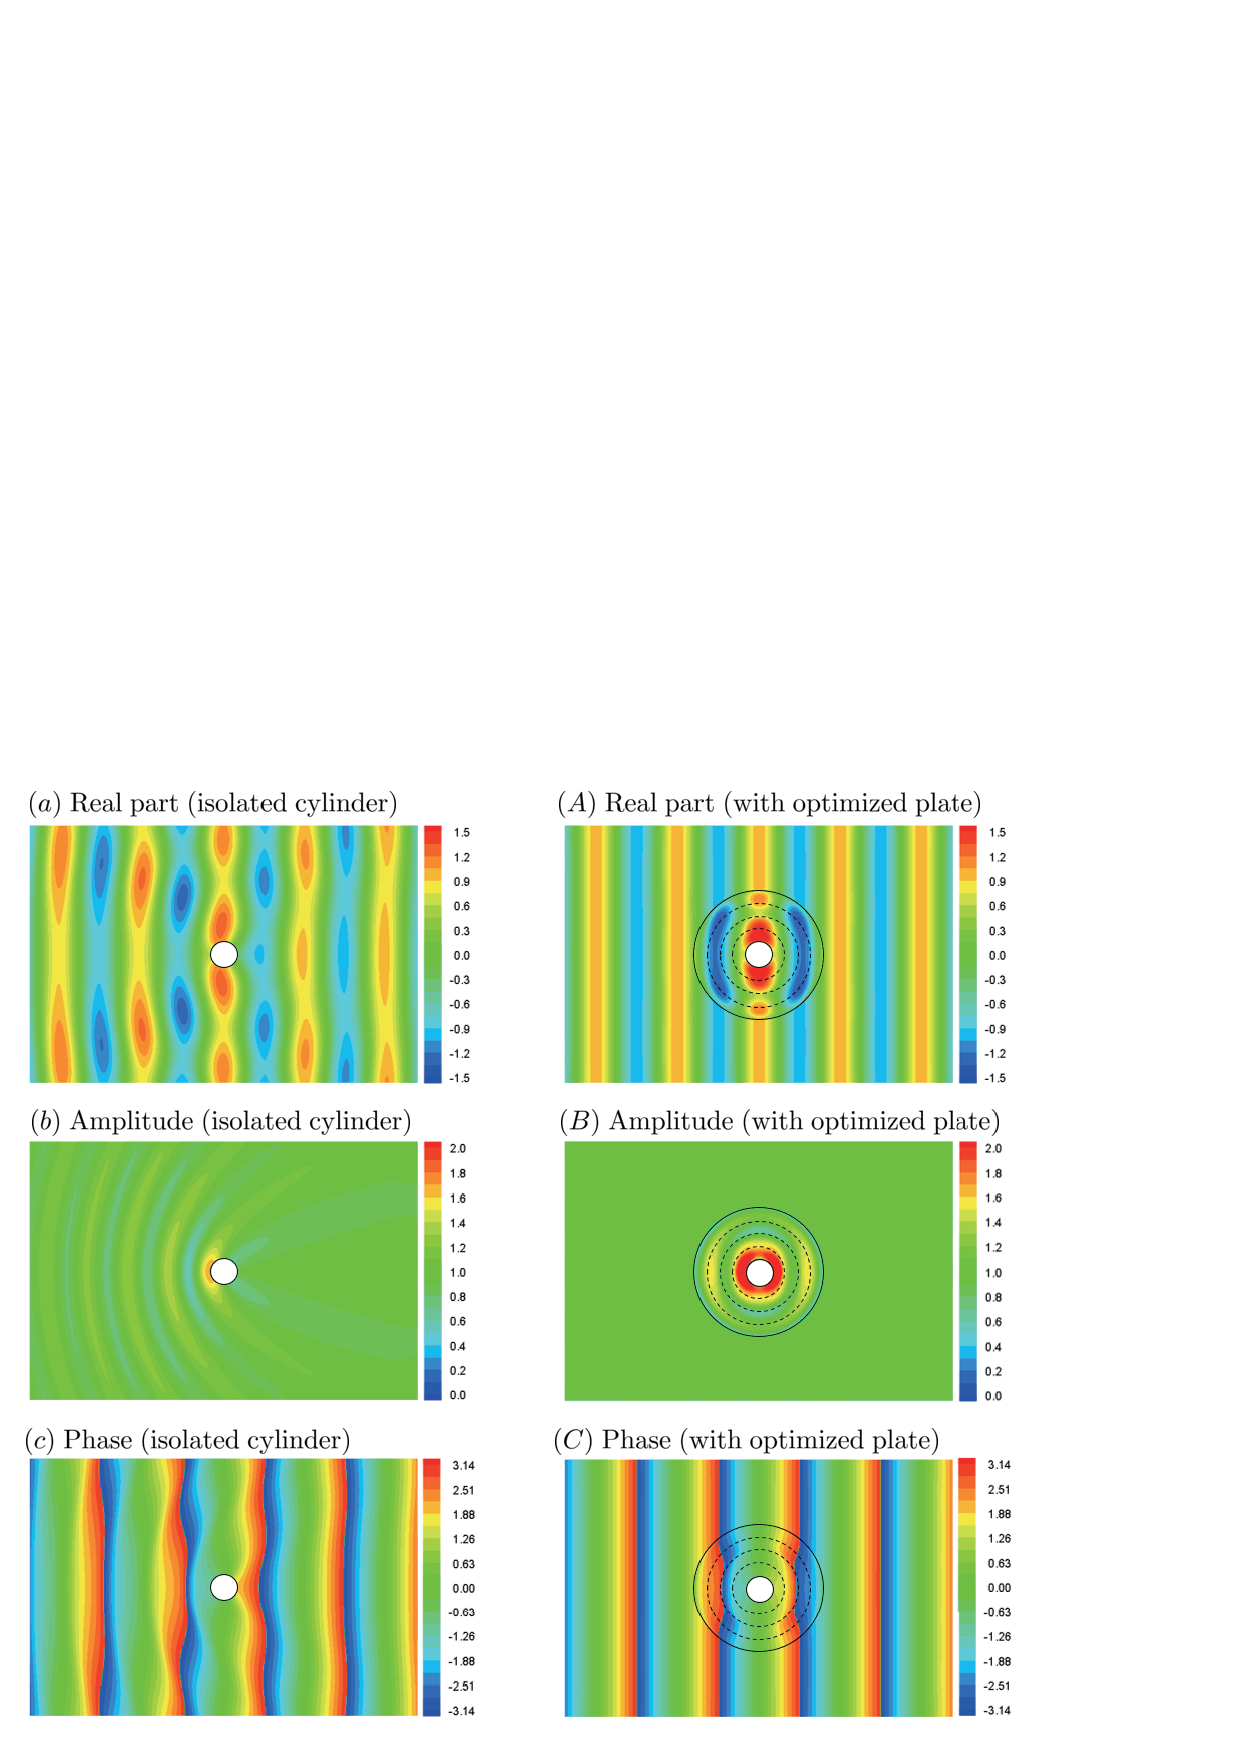
\includegraphics[width=0.99\linewidth]{figures/fig2.pdf}
\caption{Demonstration of our method over an example instance from QAsper~\cite{dasigi-etal-2021-dataset}. A long sequence is fed to a model, producing representations for the marker special tokens. Then, these vectors are used to compute our contrastive objective. The token colored in blue represents the question, and the tokens colored in green (red) represent positive (negative) evidence sentences. The goal is to maximize the similarity between the blue vector and the green vectors.}
\label{fig:model}
\end{figure*}
